%% bare_jrnl.tex
%% V1.4b
%% 2015/08/26
%% by Michael Shell
%% see http://www.michaelshell.org/
%% for current contact information.
%%
%% This is a skeleton file demonstrating the use of IEEEtran.cls
%% (requires IEEEtran.cls version 1.8b or later) with an IEEE
%% journal paper.
%%
%% Support sites:
%% http://www.michaelshell.org/tex/ieeetran/
%% http://www.ctan.org/pkg/ieeetran
%% and
%% http://www.ieee.org/

%%*************************************************************************
%% Legal Notice:
%% This code is offered as-is without any warranty either expressed or
%% implied; without even the implied warranty of MERCHANTABILITY or
%% FITNESS FOR A PARTICULAR PURPOSE! 
%% User assumes all risk.
%% In no event shall the IEEE or any contributor to this code be liable for
%% any damages or losses, including, but not limited to, incidental,
%% consequential, or any other damages, resulting from the use or misuse
%% of any information contained here.
%%
%% All comments are the opinions of their respective authors and are not
%% necessarily endorsed by the IEEE.
%%
%% This work is distributed under the LaTeX Project Public License (LPPL)
%% ( http://www.latex-project.org/ ) version 1.3, and may be freely used,
%% distributed and modified. A copy of the LPPL, version 1.3, is included
%% in the base LaTeX documentation of all distributions of LaTeX released
%% 2003/12/01 or later.
%% Retain all contribution notices and credits.
%% ** Modified files should be clearly indicated as such, including  **
%% ** renaming them and changing author support contact information. **
%%*************************************************************************


% *** Authors should verify (and, if needed, correct) their LaTeX system  ***
% *** with the testflow diagnostic prior to trusting their LaTeX platform ***
% *** with production work. The IEEE's font choices and paper sizes can   ***
% *** trigger bugs that do not appear when using other class files.       ***                          ***
% The testflow support page is at:
% http://www.michaelshell.org/tex/testflow/



\documentclass[journal]{IEEEtran}
%
% If IEEEtran.cls has not been installed into the LaTeX system files,
% manually specify the path to it like:
% \documentclass[journal]{../sty/IEEEtran}


\usepackage{pdfpages}


% Some very useful LaTeX packages include:
% (uncomment the ones you want to load)


% *** MISC UTILITY PACKAGES ***
%
%\usepackage{ifpdf}
% Heiko Oberdiek's ifpdf.sty is very useful if you need conditional
% compilation based on whether the output is pdf or dvi.
% usage:
% \ifpdf
%   % pdf code
% \else
%   % dvi code
% \fi
% The latest version of ifpdf.sty can be obtained from:
% http://www.ctan.org/pkg/ifpdf
% Also, note that IEEEtran.cls V1.7 and later provides a builtin
% \ifCLASSINFOpdf conditional that works the same way.
% When switching from latex to pdflatex and vice-versa, the compiler may
% have to be run twice to clear warning/error messages.

% *** CITATION PACKAGES ***
%
\usepackage{cite}
% cite.sty was written by Donald Arseneau
% V1.6 and later of IEEEtran pre-defines the format of the cite.sty package
% \cite{} output to follow that of the IEEE. Loading the cite package will
% result in citation numbers being automatically sorted and properly
% "compressed/ranged". e.g., [1], [9], [2], [7], [5], [6] without using
% cite.sty will become [1], [2], [5]--[7], [9] using cite.sty. cite.sty's
% \cite will automatically add leading space, if needed. Use cite.sty's
% noadjust option (cite.sty V3.8 and later) if you want to turn this off
% such as if a citation ever needs to be enclosed in parenthesis.
% cite.sty is already installed on most LaTeX systems. Be sure and use
% version 5.0 (2009-03-20) and later if using hyperref.sty.
% The latest version can be obtained at:
% http://www.ctan.org/pkg/cite
% The documentation is contained in the cite.sty file itself.

\RequirePackage[utf8]{inputenc}

% *** GRAPHICS RELATED PACKAGES ***
%
%\ifCLASSINFOpdf
  %\usepackage[pdftex]{graphicx}
  % declare the path(s) where your graphic files are
  %\graphicspath{{../pdf/}{../jpeg/}{./images/}}
  % and their extensions so you won't have to specify these with
  % every instance of \includegraphics
  %\DeclareGraphicsExtensions{.pdf,.jpeg,.png}
%\else
  % or other class option (dvipsone, dvipdf, if not using dvips). graphicx
  % will default to the driver specified in the system graphics.cfg if no
  % driver is specified.
  % \usepackage[dvips]{graphicx}
  % declare the path(s) where your graphic files are
  % \graphicspath{{../eps/}}
  % and their extensions so you won't have to specify these with
  % every instance of \includegraphics
  % \DeclareGraphicsExtensions{.eps}
%\fi
% graphicx was written by David Carlisle and Sebastian Rahtz. It is
% required if you want graphics, photos, etc. graphicx.sty is already
% installed on most LaTeX systems. The latest version and documentation
% can be obtained at: 
% http://www.ctan.org/pkg/graphicx
% Another good source of documentation is "Using Imported Graphics in
% LaTeX2e" by Keith Reckdahl which can be found at:
% http://www.ctan.org/pkg/epslatex
%
% latex, and pdflatex in dvi mode, support graphics in encapsulated
% postscript (.eps) format. pdflatex in pdf mode supports graphics
% in .pdf, .jpeg, .png and .mps (metapost) formats. Users should ensure
% that all non-photo figures use a vector format (.eps, .pdf, .mps) and
% not a bitmapped formats (.jpeg, .png). The IEEE frowns on bitmapped formats
% which can result in "jaggedy"/blurry rendering of lines and letters as
% well as large increases in file sizes.
%
% You can find documentation about the pdfTeX application at:
% http://www.tug.org/applications/pdftex





% *** MATH PACKAGES ***
%
%\usepackage{amsmath}
% A popular package from the American Mathematical Society that provides
% many useful and powerful commands for dealing with mathematics.
%
% Note that the amsmath package sets \interdisplaylinepenalty to 10000
% thus preventing page breaks from occurring within multiline equations. Use:
%\interdisplaylinepenalty=2500
% after loading amsmath to restore such page breaks as IEEEtran.cls normally
% does. amsmath.sty is already installed on most LaTeX systems. The latest
% version and documentation can be obtained at:
% http://www.ctan.org/pkg/amsmath





% *** SPECIALIZED LIST PACKAGES ***
%
%\usepackage{algorithmic}
% algorithmic.sty was written by Peter Williams and Rogerio Brito.
% This package provides an algorithmic environment fo describing algorithms.
% You can use the algorithmic environment in-text or within a figure
% environment to provide for a floating algorithm. Do NOT use the algorithm
% floating environment provided by algorithm.sty (by the same authors) or
% algorithm2e.sty (by Christophe Fiorio) as the IEEE does not use dedicated
% algorithm float types and packages that provide these will not provide
% correct IEEE style captions. The latest version and documentation of
% algorithmic.sty can be obtained at:
% http://www.ctan.org/pkg/algorithms
% Also of interest may be the (relatively newer and more customizable)
% algorithmicx.sty package by Szasz Janos:
% http://www.ctan.org/pkg/algorithmicx




% *** ALIGNMENT PACKAGES ***
%
%\usepackage{array}
% Frank Mittelbach's and David Carlisle's array.sty patches and improves
% the standard LaTeX2e array and tabular environments to provide better
% appearance and additional user controls. As the default LaTeX2e table
% generation code is lacking to the point of almost being broken with
% respect to the quality of the end results, all users are strongly
% advised to use an enhanced (at the very least that provided by array.sty)
% set of table tools. array.sty is already installed on most systems. The
% latest version and documentation can be obtained at:
% http://www.ctan.org/pkg/array


% IEEEtran contains the IEEEeqnarray family of commands that can be used to
% generate multiline equations as well as matrices, tables, etc., of high
% quality.




% *** SUBFIGURE PACKAGES ***
%\ifCLASSOPTIONcompsoc
%  \usepackage[caption=false,font=normalsize,labelfont=sf,textfont=sf]{subfig}
%\else
%  \usepackage[caption=false,font=footnotesize]{subfig}
%\fi
% subfig.sty, written by Steven Douglas Cochran, is the modern replacement
% for subfigure.sty, the latter of which is no longer maintained and is
% incompatible with some LaTeX packages including fixltx2e. However,
% subfig.sty requires and automatically loads Axel Sommerfeldt's caption.sty
% which will override IEEEtran.cls' handling of captions and this will result
% in non-IEEE style figure/table captions. To prevent this problem, be sure
% and invoke subfig.sty's "caption=false" package option (available since
% subfig.sty version 1.3, 2005/06/28) as this is will preserve IEEEtran.cls
% handling of captions.
% Note that the Computer Society format requires a larger sans serif font
% than the serif footnote size font used in traditional IEEE formatting
% and thus the need to invoke different subfig.sty package options depending
% on whether compsoc mode has been enabled.
%
% The latest version and documentation of subfig.sty can be obtained at:
% http://www.ctan.org/pkg/subfig




% *** FLOAT PACKAGES ***
%
%\usepackage{fixltx2e}
% fixltx2e, the successor to the earlier fix2col.sty, was written by
% Frank Mittelbach and David Carlisle. This package corrects a few problems
% in the LaTeX2e kernel, the most notable of which is that in current
% LaTeX2e releases, the ordering of single and double column floats is not
% guaranteed to be preserved. Thus, an unpatched LaTeX2e can allow a
% single column figure to be placed prior to an earlier double column
% figure.
% Be aware that LaTeX2e kernels dated 2015 and later have fixltx2e.sty's
% corrections already built into the system in which case a warning will
% be issued if an attempt is made to load fixltx2e.sty as it is no longer
% needed.
% The latest version and documentation can be found at:
% http://www.ctan.org/pkg/fixltx2e


%\usepackage{stfloats}
% stfloats.sty was written by Sigitas Tolusis. This package gives LaTeX2e
% the ability to do double column floats at the bottom of the page as well
% as the top. (e.g., "\begin{figure*}[!b]" is not normally possible in
% LaTeX2e). It also provides a command:
%\fnbelowfloat
% to enable the placement of footnotes below bottom floats (the standard
% LaTeX2e kernel puts them above bottom floats). This is an invasive package
% which rewrites many portions of the LaTeX2e float routines. It may not work
% with other packages that modify the LaTeX2e float routines. The latest
% version and documentation can be obtained at:
% http://www.ctan.org/pkg/stfloats
% Do not use the stfloats baselinefloat ability as the IEEE does not allow
% \baselineskip to stretch. Authors submitting work to the IEEE should note
% that the IEEE rarely uses double column equations and that authors should try
% to avoid such use. Do not be tempted to use the cuted.sty or midfloat.sty
% packages (also by Sigitas Tolusis) as the IEEE does not format its papers in
% such ways.
% Do not attempt to use stfloats with fixltx2e as they are incompatible.
% Instead, use Morten Hogholm'a dblfloatfix which combines the features
% of both fixltx2e and stfloats:
%
% \usepackage{dblfloatfix}
% The latest version can be found at:
% http://www.ctan.org/pkg/dblfloatfix




%\ifCLASSOPTIONcaptionsoff
%  \usepackage[nomarkers]{endfloat}
% \let\MYoriglatexcaption\caption
% \renewcommand{\caption}[2][\relax]{\MYoriglatexcaption[#2]{#2}}
%\fi
% endfloat.sty was written by James Darrell McCauley, Jeff Goldberg and 
% Axel Sommerfeldt. This package may be useful when used in conjunction with 
% IEEEtran.cls'  captionsoff option. Some IEEE journals/societies require that
% submissions have lists of figures/tables at the end of the paper and that
% figures/tables without any captions are placed on a page by themselves at
% the end of the document. If needed, the draftcls IEEEtran class option or
% \CLASSINPUTbaselinestretch interface can be used to increase the line
% spacing as well. Be sure and use the nomarkers option of endfloat to
% prevent endfloat from "marking" where the figures would have been placed
% in the text. The two hack lines of code above are a slight modification of
% that suggested by in the endfloat docs (section 8.4.1) to ensure that
% the full captions always appear in the list of figures/tables - even if
% the user used the short optional argument of \caption[]{}.
% IEEE papers do not typically make use of \caption[]'s optional argument,
% so this should not be an issue. A similar trick can be used to disable
% captions of packages such as subfig.sty that lack options to turn off
% the subcaptions:
% For subfig.sty:
% \let\MYorigsubfloat\subfloat
% \renewcommand{\subfloat}[2][\relax]{\MYorigsubfloat[]{#2}}
% However, the above trick will not work if both optional arguments of
% the \subfloat command are used. Furthermore, there needs to be a
% description of each subfigure *somewhere* and endfloat does not add
% subfigure captions to its list of figures. Thus, the best approach is to
% avoid the use of subfigure captions (many IEEE journals avoid them anyway)
% and instead reference/explain all the subfigures within the main caption.
% The latest version of endfloat.sty and its documentation can obtained at:
% http://www.ctan.org/pkg/endfloat
%
% The IEEEtran \ifCLASSOPTIONcaptionsoff conditional can also be used
% later in the document, say, to conditionally put the References on a 
% page by themselves.




% *** PDF, URL AND HYPERLINK PACKAGES ***
%
\usepackage{url}

% url.sty was written by Donald Arseneau. It provides better support for
% handling and breaking URLs. url.sty is already installed on most LaTeX
% systems. The latest version and documentation can be obtained at:
% http://www.ctan.org/pkg/url
% Basically, \url{my_url_here}.




% *** Do not adjust lengths that control margins, column widths, etc. ***
% *** Do not use packages that alter fonts (such as pslatex).         ***
% There should be no need to do such things with IEEEtran.cls V1.6 and later.
% (Unless specifically asked to do so by the journal or conference you plan
% to submit to, of course. )


% correct bad hyphenation here
%\hyphenation{op-tical net-works semi-conduc-tor}


\begin{document}
%
% paper title
% Titles are generally capitalized except for words such as a, an, and, as,
% at, but, by, for, in, nor, of, on, or, the, to and up, which are usually
% not capitalized unless they are the first or last word of the title.
% Linebreaks \\ can be used within to get better formatting as desired.
% Do not put math or special symbols in the title.
\title{Breaking Text-based CAPTCHAs with Convolutional Neural Networks}
%
%
% author names and IEEE memberships
% note positions of commas and nonbreaking spaces ( ~ ) LaTeX will not break
% a structure at a ~ so this keeps an author's name from being broken across
% two lines.
% use \thanks{} to gain access to the first footnote area
% a separate \thanks must be used for each paragraph as LaTeX2e's \thanks
% was not built to handle multiple paragraphs
%

%\author{Michael~Shell,~\IEEEmembership{Member,~IEEE,}
  %      John~Doe,~\IEEEmembership{Fellow,~OSA,}
    %    and~Jane~Doe,~\IEEEmembership{Life~Fellow,~IEEE}% <-this % stops a space
%\thanks{M. Shell was with the Department
%of Electrical and Computer Engineering, Georgia Institute of Technology, Atlanta,
%GA, 30332 USA e-mail: (see http://www.michaelshell.org/contact.html).}% <-this % stops a space
%\thanks{J. Doe and J. Doe are with Anonymous University.}% <-this % stops a space
%\thanks{Manuscript received April 19, 2005; revised August 26, 2015.}}
\author{ Diogo Daniel Ferreira, Luís Leira \\
Department of Electronic, Telecommunications and Informatics \\
University of Aveiro}


% note the % following the last \IEEEmembership and also \thanks - 
% these prevent an unwanted space from occurring between the last author name
% and the end of the author line. i.e., if you had this:
% 
% \author{....lastname \thanks{...} \thanks{...} }
%                     ^------------^------------^----Do not want these spaces!
%
% a space would be appended to the last name and could cause every name on that
% line to be shifted left slightly. This is one of those "LaTeX things". For
% instance, "\textbf{A} \textbf{B}" will typeset as "A B" not "AB". To get
% "AB" then you have to do: "\textbf{A}\textbf{B}"
% \thanks is no different in this regard, so shield the last } of each \thanks
% that ends a line with a % and do not let a space in before the next \thanks.
% Spaces after \IEEEmembership other than the last one are OK (and needed) as
% you are supposed to have spaces between the names. For what it is worth,
% this is a minor point as most people would not even notice if the said evil
% space somehow managed to creep in.



% The paper headers
% \markboth{Journal of \LaTeX\ Class Files,~Vol.~14, No.~8, August~2015}%
% {Shell \MakeLowercase{\textit{et al.}}: Bare Demo of IEEEtran.cls for IEEE Journals}
% The only time the second header will appear is for the odd numbered pages
% after the title page when using the twoside option.
% 
% *** Note that you probably will NOT want to include the author's ***
% *** name in the headers of peer review papers.                   ***
% You can use \ifCLASSOPTIONpeerreview for conditional compilation here if
% you desire.




% If you want to put a publisher's ID mark on the page you can do it like
% this:
%\IEEEpubid{0000--0000/00\$00.00~\copyright~2015 IEEE}
% Remember, if you use this you must call \IEEEpubidadjcol in the second
% column for its text to clear the IEEEpubid mark.



% use for special paper notices
%\IEEEspecialpapernotice{(Invited Paper)}

% make the title area
\maketitle

% As a general rule, do not put math, special symbols or citations
% in the abstract or keywords.
\begin{abstract}
CAPTCHAs are essential for service providers to separate the human users from bots. In 2014 text-based CAPTCHAs were considered insecure and other approaches were explored, mainly relying on object recognition. However, many websites still use text-based CAPTCHAs as the main way to distinguish humans from machines.

In this report, it will be shown how to break a text-based CAPTCHA by automatically reading the characters in the image. It is performed image transformation to remove the noise in the image, character segmentation to extract the characters and different approaches are taken to the construction of a model capable of recognizing each character. This report focuses particularly on the construction of a Convolutional Neural Network with different techniques to improve its accuracy.

After the network being trained, it is also visualized the learning done by the convolutional layers with three particular techniques: Calculation of the activations of the convolutional layers given an input image, visualization of the patterns that the convolutional layers are detecting and creation of heat maps to detect what part of the character is most important for the classification made.

In the dataset used, our model achieves an accuracy of 93.91\% in character recognition, proving that with an accurate character segmentation and robust noise removal techniques applied to the images, the text-based CAPTCHAs can be broken by a machine.
\end{abstract}

% Note that keywords are not normally used for peerreview papers.
%\begin{IEEEkeywords}
%IEEE, IEEEtran, journal, \LaTeX, paper, template.
%\end{IEEEkeywords}

% For peer review papers, you can put extra information on the cover
% page as needed:
% \ifCLASSOPTIONpeerreview
% \begin{center} \bfseries EDICS Category: 3-BBND \end{center}
% \fi
%
% For peerreview papers, this IEEEtran command inserts a page break and
% creates the second title. It will be ignored for other modes.
\IEEEpeerreviewmaketitle

\section{Introduction}

\IEEEPARstart{C}{aptcha} (Completely Automated Public Turing Test to tell Computers and Humans Apart) is an automated test designed to check if the user is human. That test is made using a challenge-response approach, where the challenge is easy for a human to solve, but hard for a machine. If the response is correct, the machine assumes that the user is human.

CAPTCHAs are used by most service providers, such as email or online shopping, to prevent bots from abusing their online services. For example, to prevent a botnet to create hundreds of new email accounts per second, a CAPTCHA can be used to assure that the users creating the email accounts are humans.

The construction of CAPTCHAs is hard because it is uneasy to create challenges hard for machines but easily solvable by humans. Over the years, the most used CAPTCHAs are based on visual-perception tasks. Usually, are presented distorted characters that must be typed correctly by the user. Most of the times, it is also added background and foreground noise to the created CAPTCHAs, making it almost impossible for a computer to automatically recognize the characters. However, for humans, the characters are usually recognizable, due to our brain's capacity for recognizing patterns.

There are three characteristics for a modern text-based CAPTCHA to be resilient \cite{wiki:captcha}:
\begin{itemize}
    \item The large variation in the shape of letters. While there is an infinite variety of versions for the same character that the human brain can recognize, the same is not true for a computer. If all the versions of a character are different, it is hard for a computer to recognize any version not previously seen.
    \item Due to the large variation in the shape of characters, it can also be hard to perform segmentation for each character, mainly when the characters have no space in between.
    \item In specific CAPTCHAs, the context may be the key to answer correctly to the task. When the word is taken into context, it is easier for a human to answer what are the characters in the challenge, even if some of them are dubious.
\end{itemize}

The conjugation of these three characteristics makes a CAPTCHA hard to solve by a machine. In 2014, the authors of \cite{185128} concluded that text distortion-based CAPTCHAs schemes should be considered insecure due to technological advances. Since then, alternative CAPTCHA schemas based on object recognition were proposed (\cite{Sivakorn2016}, \cite{Zhao:2018:TES:3270101.3270104}), making it harder for machines to solve them, but remaining easily solvable by humans.

However, there are still many implementations of insecure text-based CAPTCHAs on the web. This report explains a possible attack that can be made to a text-based CAPTCHA. It focuses on the pre-processing and optical character recognition (OCR) of characters in a text-based CAPTCHA, exploiting different techniques to achieve higher accuracy on the OCR task.


\section{Related Work}

The majority of the CAPTCHAs used in service providers is text-based. Accordingly, there is a lot of research showing the flaws of the text-based CAPTCHAs.

In \cite{Mori}, the authors propose two algorithms for text-based CAPTCHA recognition, based on pattern matching and hierarchical algorithms. Both algorithms try to find the shape of the objects by defining key points in their structure using the Canny Edge Detector and then comparing it to the structure of each character in a local database. One algorithm is bottom-up, tries to find words in images starting with visual cues, and incorporates lexical information later (the CAPTCHAs text is words from the dictionary). The second algorithm tries to find entire words at once. The second algorithm gave better results, with an accuracy of 92\% on the EZ-Gimpy dataset and 33\% accuracy on the Gimpy dataset. This study showed that, in most cases, algorithms that deal with the whole CAPTCHA at once usually achieve higher accuracy than algorithms that deal with each character separately. The authors also said that while this technique can be effective for text-based CAPTCHAs, it is no longer effective for object recognition, due to the various shapes of objects in the world, and suggested object-based CAPTCHAs for higher complexity.

In \cite{Yan:2008:LAM:1455770.1455839}, the authors break the Microsoft CAPTCHA, used for systems such as MSN or Hotmail, with image segmentation and pattern matching. The image segmentation task achieves 92\% accuracy, and the segmentation and recognition combined have an accuracy of 60\%. Other approaches, such as \cite{Yan2007} or \cite{Li:2010:BEC:1920261.1920288}, also use image segmentation and pattern matching to break specific CAPTCHAs dataset.

In \cite{NIPS2004_2571}, the authors propose a two-step approach to recognize text-based CAPTCHAs. The dataset used includes CAPTCHAs from the most visited websites, like MSN, Yahoo!, Google/Gmail or TicketMaster, and a language model was not used to help with the recognition. First, segmentation is used to separate the characters on the CAPTCHAs. The next step is recognizing each character, using a Convolutional Neural Network. It was shown that the recognition had high accuracy when the segmentation was done right, and most of the errors derive from a bad segmentation.

In \cite{Stark_captcharecognition}, a Convolutional Neural Network (CNN) is used for CAPTCHA recognition. The network is composed by three convolution layers, three pooling layers and two fully-connected layers. The network recognizes the sequence without pre-segmentation, and with a fixed size of six characters. The problem of CNN requiring a very large training set is solved with an Active Learning mechanism. To prevent from feeding the neural network millions of CAPTCHAs, each CAPTCHA is recognized with a certain measured uncertainty. Only the most uncertain CAPTCHAs on the test set are used for retraining the model. The algorithm reaches an accuracy of almost 90\%.

In \cite{George2017}, a novel approach is taken to break text-based CAPTCHAs. It is introduced the Recursive Cortical Network (RCN), a hierarchical probabilistic generative model with an outstanding capacity of generalization based on the human brain, designed to be trained with few examples. This model achieved an accuracy of 94.3\% on character recognition on the reCAPTCHA algorithm, created and currently used by Google.

In \cite{185128}, the authors present a general framework for solving text-based CAPTCHAs, with a multi-step algorithm based on reinforcement learning with joint phases of segmentation and recognition, for better results in both steps.


\section{Dataset}

The dataset used in this work is from Kaggle Website\footnote{\url{https://www.kaggle.com/fournierp/captcha-version-2-images}}. It contains 1070 text-based CAPTCHAs. These CAPTCHAs contain five of the following 19 characters: 2, 3, 4, 5, 6, 7, 8, b, c, d, e, f, g, m, n, p, w, x, y.

The dataset has several important characteristics to be mentioned. Each CAPTCHA has exactly five random characters, with no relation among them (the characters do not form a word). There is noise in the CAPTCHAs, mainly in the form of black lines over the black characters. It can also be seen that the characters are approximately in the same position for every image, which eases the process of segmentation. The characters have the same font across all CAPTCHAs, but they are rotated in different angles. Twenty samples from the dataset can be seen in figure \ref{captchas_example}.

\begin{figure}[!t]
\centering
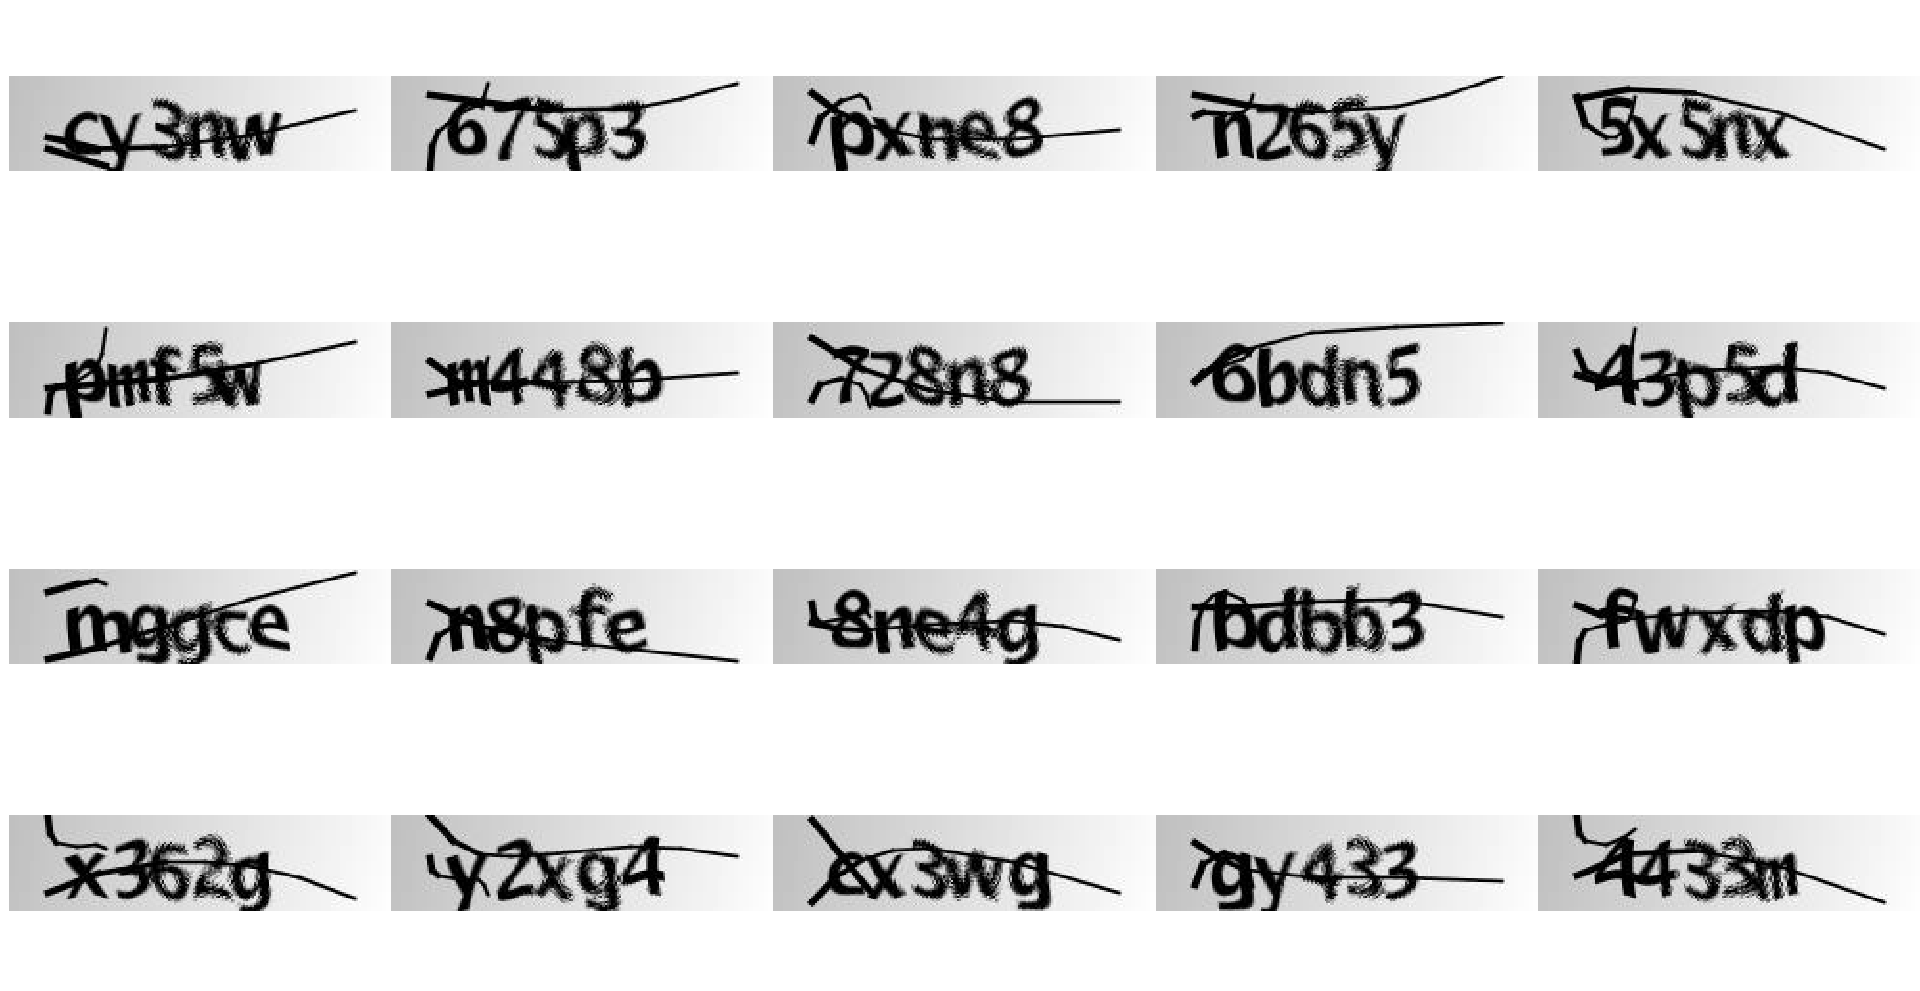
\includegraphics[width=3in]{images/captcha_extraction}
\caption{20 samples from the CAPTCHA dataset.}
\label{captchas_example}
\end{figure}


\section{Image pre-processing}

To ease the classification method, the CAPTCHAs will be divided into characters, turning the problem into a classic OCR problem. Before the segmentation, a few steps are taken to remove or alleviate the background noise. First, it is applied the Otsu method to perform clustering-based image thresholding to assure that the CAPTCHA is a binary image. Then, a sequence of morphological transformations is applied to the image. A dilation and an erosion are applied sequentially, using a kernel of 3x3. Finally, another dilation is applied with a kernel of 3x1, in an attempt to eliminate the horizontal lines that create the noise in the image. After all image operations, the characters are extracted from the CAPTCHA using pre-determined pixel coordinates. After human analysis, it was determined that the extracted characters had a size of 21w x 38h. The transformations applied to the CAPTCHAs are depicted in figure \ref{image_transformations}.

\begin{figure}[!t]
\centering
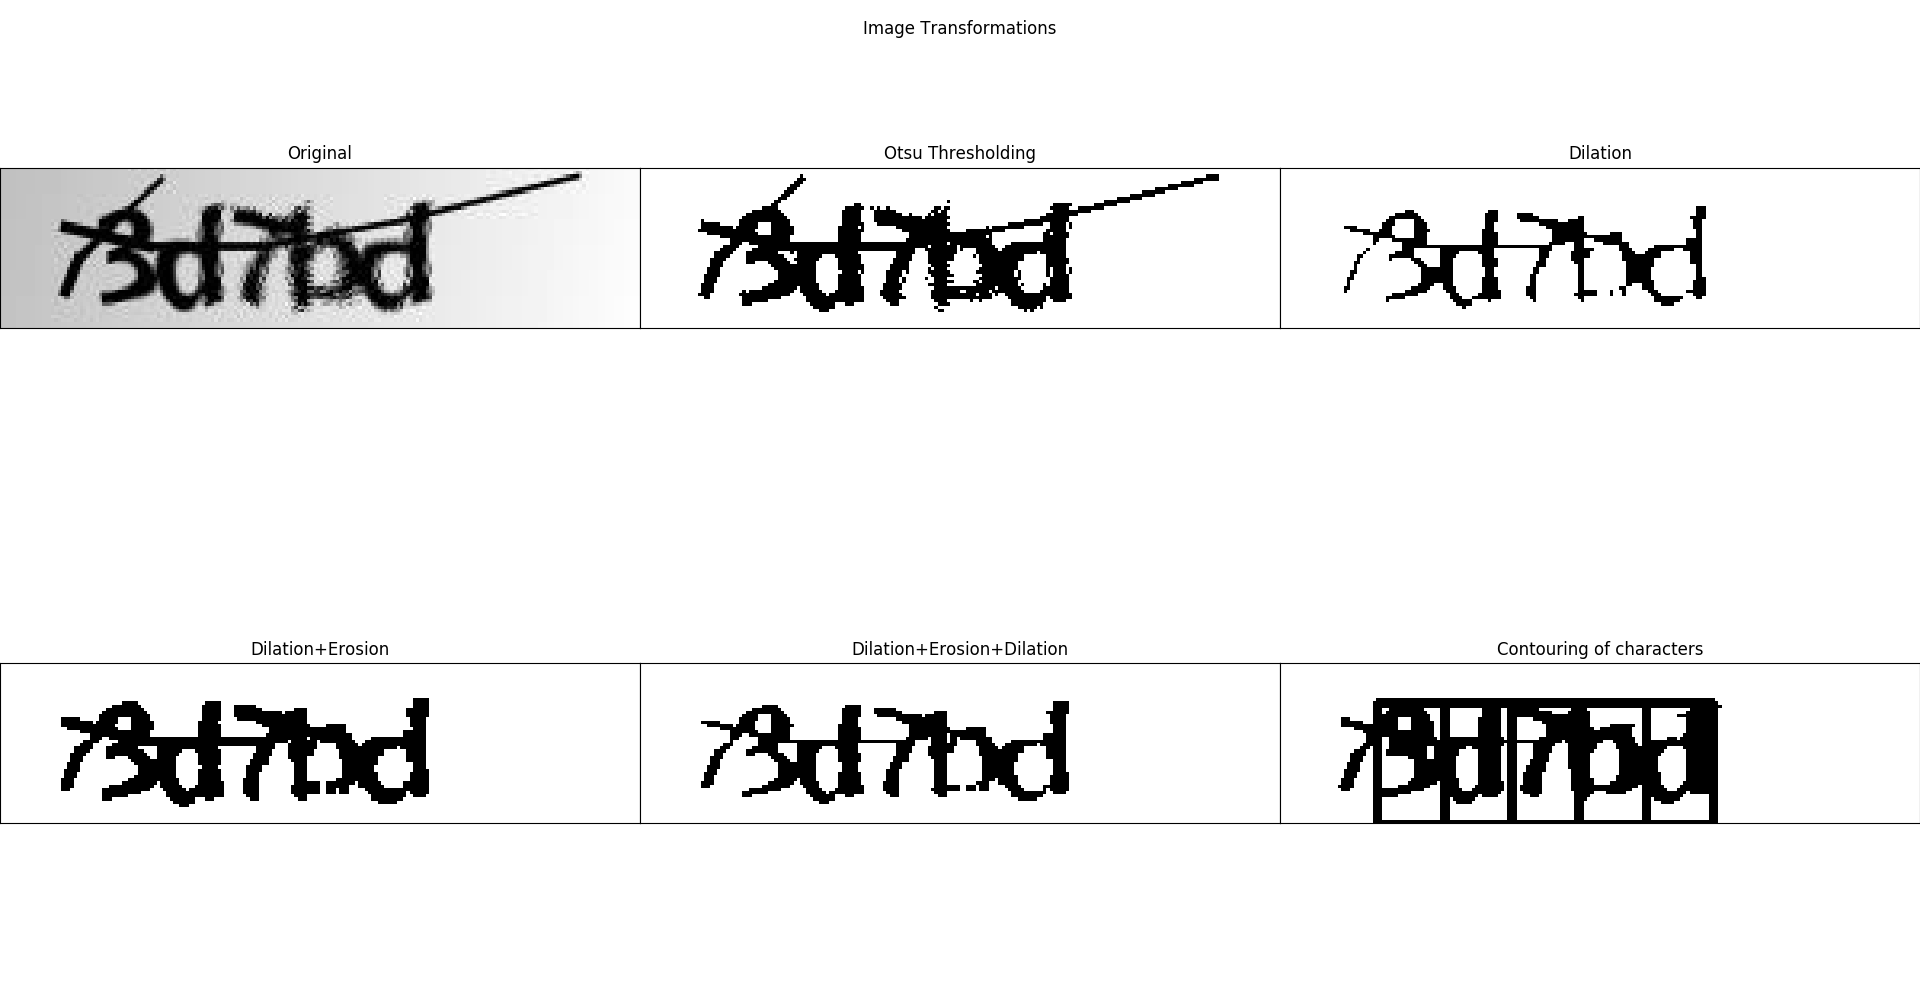
\includegraphics[width=3in]{images/image_Transformations}
\caption{Transformations applied to CAPTCHAs to remove the noise. On the top, from left to right, it can be seen the original image, the image after the Otsu thresholding and the image after one dilation. On the bottom, from left to right, it can be seen the image after the erosion, the image after the second dilation and finally the contouring of the characters.}
\label{image_transformations}
\end{figure}

The characters have the frequency shown in table \ref{table:character_frequency} and a sample of each class of characters can be seen in figure \ref{characters_extraction}.

\begin{table}[]
\centering
\caption{Character frequency in the dataset.}
\label{table:character_frequency}
\begin{tabular}{|l|l|}
\hline
Character & Frequency \\ \hline
2         & 270       \\ \hline
3         & 271       \\ \hline
4         & 289       \\ \hline
5         & 288       \\ \hline
6         & 267       \\ \hline
7         & 262       \\ \hline
8         & 272       \\ \hline
b         & 247       \\ \hline
c         & 276       \\ \hline
d         & 268       \\ \hline
e         & 245       \\ \hline
f         & 277       \\ \hline
g         & 281       \\ \hline
m         & 282       \\ \hline
n         & 541       \\ \hline
p         & 259       \\ \hline
w         & 244       \\ \hline
x         & 271       \\ \hline
y         & 240       \\ \hline
\end{tabular}
\end{table}

As can be seen, almost all characters have a similar frequency, with the exception of the character 'n', that has approximately double the frequency of the other characters. For each character, the images were divided following rule: 60\% of the dataset of each character was for training, 20\% for cross-validation and 20\% for test.

\begin{figure}[!t]
\centering
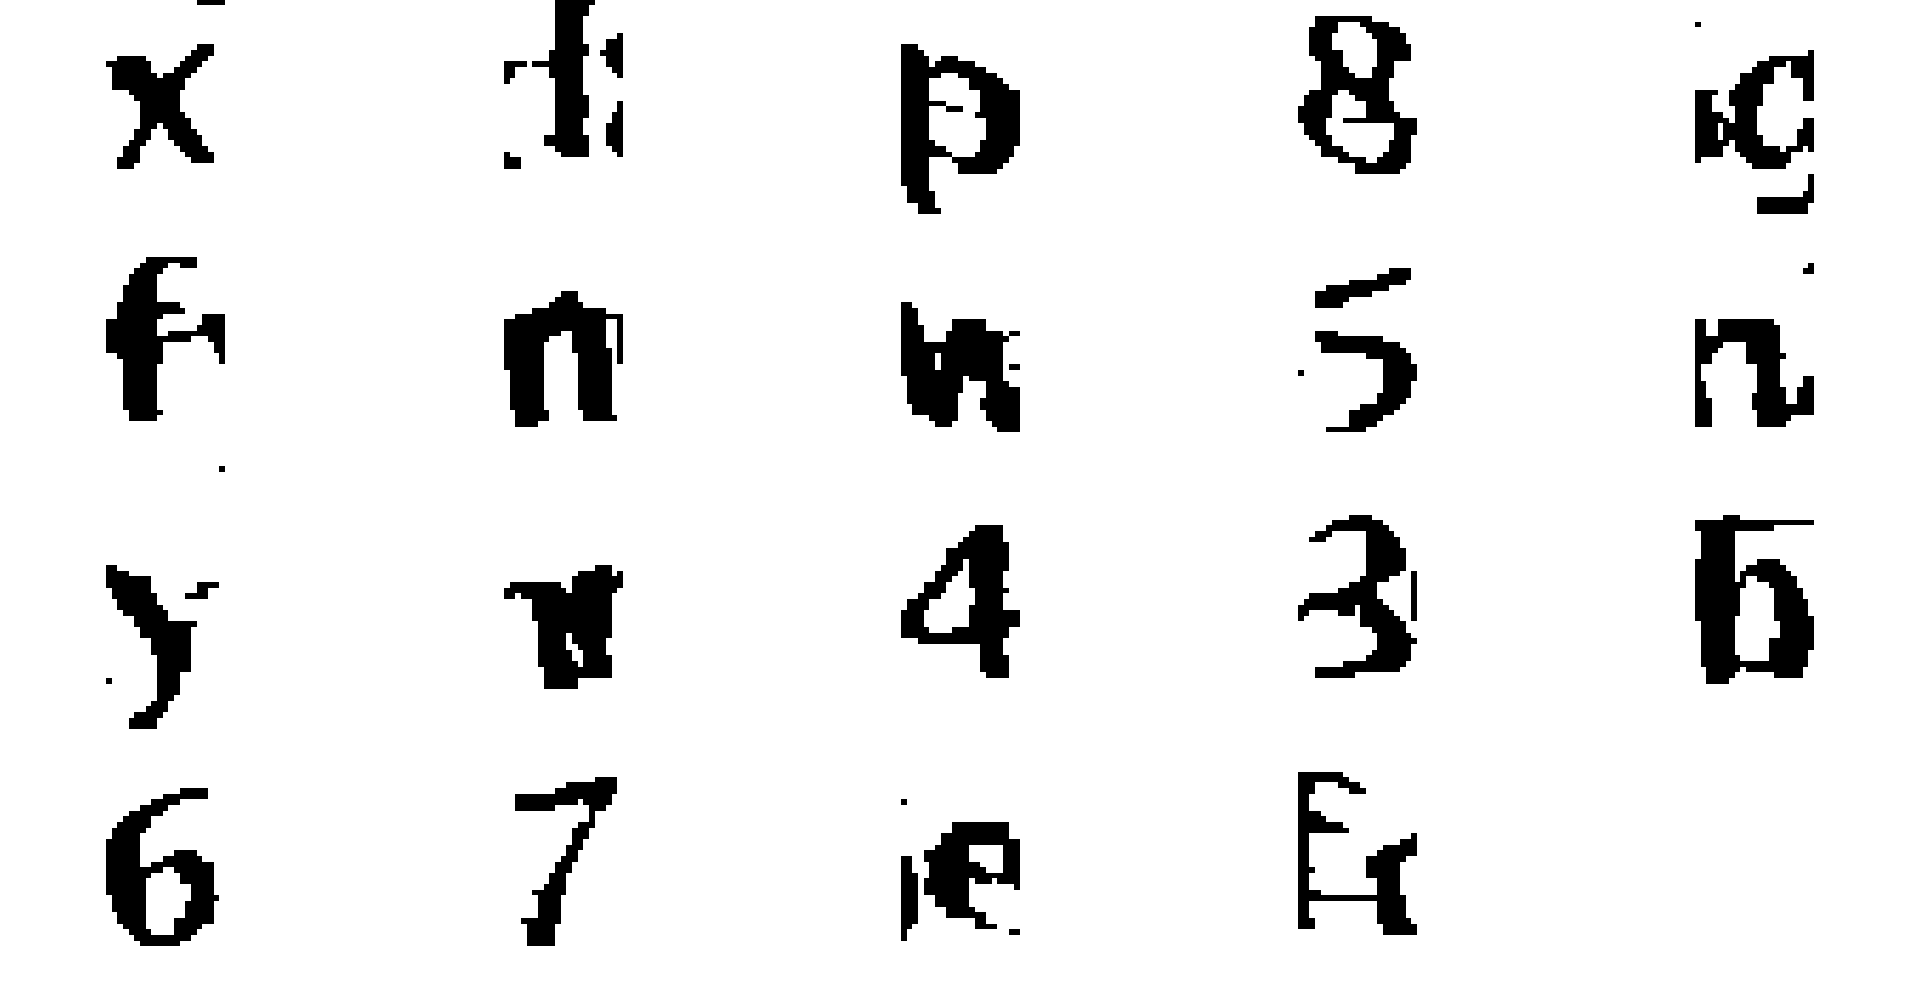
\includegraphics[width=3in]{images/character_extraction}
\caption{One sample for each one of the 19 classes of characters extracted.}
\label{characters_extraction}
\end{figure}


\section{Experiments and Results}

\subsection{Training with original CAPTCHAs dataset}

The first approach to achieve a model to classify the CAPTCHA characters was trained with the training set of the CAPTCHA dataset and validated with the cross-validation set. Various Convolutional Neural Network models were tested with different configurations. 

Initially, the Adam optimizer was used but gave poor results, as it can be seen in figure \ref{results_1}, with a maximum accuracy on the cross-validation set of 10.16\%. The optimizer used was stochastic gradient descent with a learning rate of 0.0001. The chosen loss function was categorical cross-entropy. All layers have the ReLu (Rectified Linear Unit) as activation function, except the last layer, that has the softmax function as activation function. The network configuration is described in table \ref{table:network_configuration_first}.

\begin{table}[]
\centering
\caption{First network configuration.}
\label{table:network_configuration_first}
\begin{tabular}{|l|l|l|}
\hline
\textbf{Layer Type}   & \textbf{Neurons} & \textbf{Kernel Size} \\ \hline
Convolutional Layer   & 256              & 3x3                  \\ \hline
Convolutional Layer   & 256              & 3x3                  \\ \hline
Pooling Layer         &                  & 2x2                  \\ \hline
Convolutional Layer   & 512              & 3x3                  \\ \hline
Convolutional Layer   & 512              & 3x3                  \\ \hline
Pooling Layer         &                  & 2x2                  \\ \hline
Fully-connected Layer & 512              &                      \\ \hline
Fully-connected Layer & 512              &                      \\ \hline
Fully-connected Layer & 512              &                      \\ \hline
Output Layer          & 19               &                      \\ \hline
\end{tabular}
\end{table}

\begin{figure}[!t]
\centering
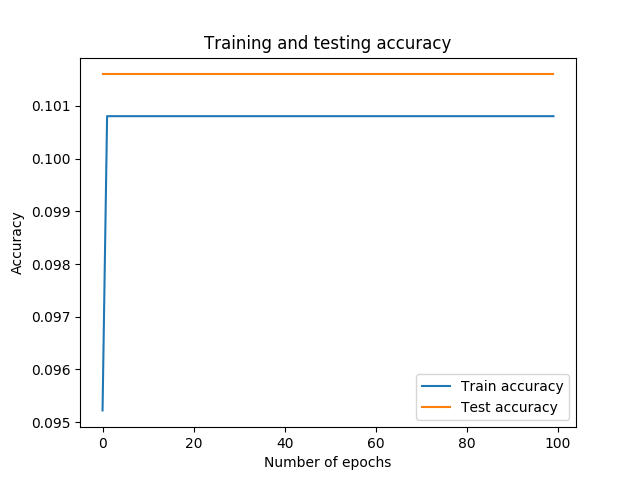
\includegraphics[width=3in]{images/test_1}
\caption{Training and cross-validation accuracy with Adam as optimizer.}
\label{results_1}
\end{figure}

With the stochastic gradient descent, it achieves better results than with the Adam optimizer accordingly to figures \ref{results_2} and \ref{results_2}. With this network, it was achieved maximum accuracy of 88.52\% on the cross-validation set.

\begin{figure}[!t]
\centering
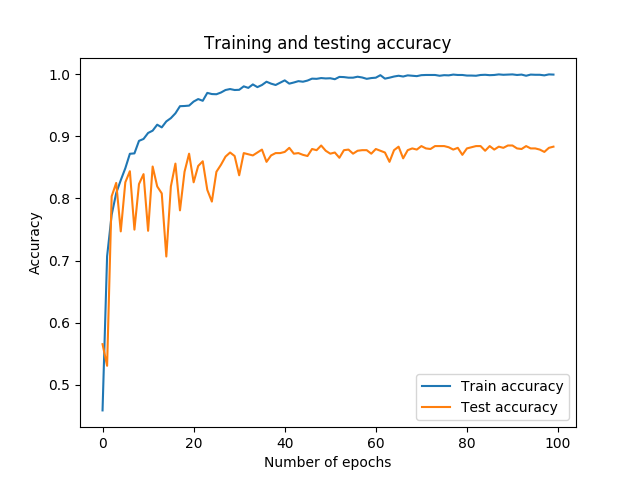
\includegraphics[width=3in]{images/test_2}
\caption{Training and cross-validation accuracy with the Stochastic Gradient Descent as optimizer.}
\label{results_2}
\end{figure}

To prevent over-fitting and improve the general accuracy, they were added three dropout layers to the network, with the value of 25\%. The new network configuration is described in table \ref{table:network_configuration_second} and the results can be seen in figure \ref{results_3}. The accuracy on the cross-validation set improved to 92.00\%.

\begin{figure}[!t]
\centering
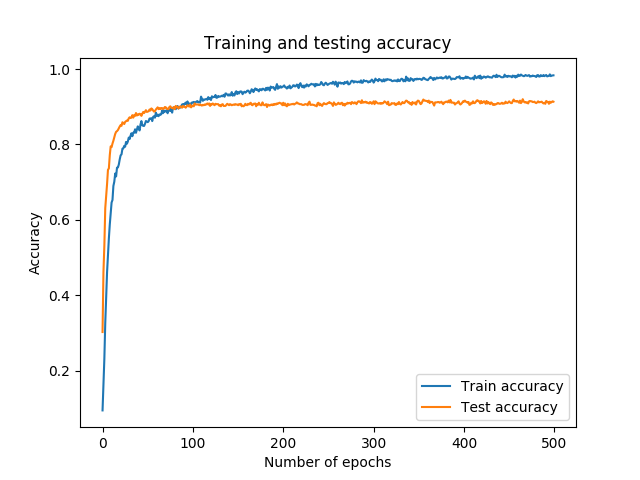
\includegraphics[width=3in]{images/test_3}
\caption{Training and cross-validation accuracy with a dropout of 25\%.}
\label{results_3}
\end{figure}

\begin{table}[]
\centering
\caption{Second network configuration. Dropout was added to improve regularization.}
\label{table:network_configuration_second}
\begin{tabular}{|l|l|l|}
\hline
\textbf{Layer Type}   & \textbf{Neurons} & \textbf{Kernel Size} \\ \hline
Convolutional Layer   & 256              & 3x3                  \\ \hline
Convolutional Layer   & 256              & 3x3                  \\ \hline
Pooling Layer         &                  & 2x2                  \\ \hline
Dropout (0.25)        &                  &                      \\ \hline
Convolutional Layer   & 512              & 3x3                  \\ \hline
Convolutional Layer   & 512              & 3x3                  \\ \hline
Pooling Layer         &                  & 2x2                  \\ \hline
Dropout (0.25)        &                  &                      \\ \hline
Fully-connected Layer & 512              &                      \\ \hline
Fully-connected Layer & 512              &                      \\ \hline
Dropout (0.25)        &                  &                      \\ \hline
Fully-connected Layer & 512              &                      \\ \hline
Output Layer          & 19               &                      \\ \hline
\end{tabular}
\end{table}

In the next model, the network configuration is the same as in the table \ref{table:network_configuration_second}, but the dropout value is higher (50\%), as can be seen in the table \ref{table:network_configuration_best}. The results can be seen in the image \ref{results_4}. The maximum accuracy on the cross-validation set did not change from the previous experiment (92.00\%).

\begin{table}[]
\centering
\caption{Third network configuration. Dropout value was doubled over the previous.}
\label{table:network_configuration_best}
\begin{tabular}{|l|l|l|}
\hline
\textbf{Layer Type}   & \textbf{Neurons} & \textbf{Kernel Size} \\ \hline
Convolutional Layer   & 256              & 3x3                  \\ \hline
Convolutional Layer   & 256              & 3x3                  \\ \hline
Pooling Layer         &                  & 2x2                  \\ \hline
Dropout (0.50)        &                  &                      \\ \hline
Convolutional Layer   & 512              & 3x3                  \\ \hline
Convolutional Layer   & 512              & 3x3                  \\ \hline
Pooling Layer         &                  & 2x2                  \\ \hline
Dropout (0.50)        &                  &                      \\ \hline
Fully-connected Layer & 512              &                      \\ \hline
Fully-connected Layer & 512              &                      \\ \hline
Dropout (0.5o)        &                  &                      \\ \hline
Fully-connected Layer & 512              &                      \\ \hline
Output Layer          & 19               &                      \\ \hline
\end{tabular}
\end{table}

\begin{figure}[!t]
\centering
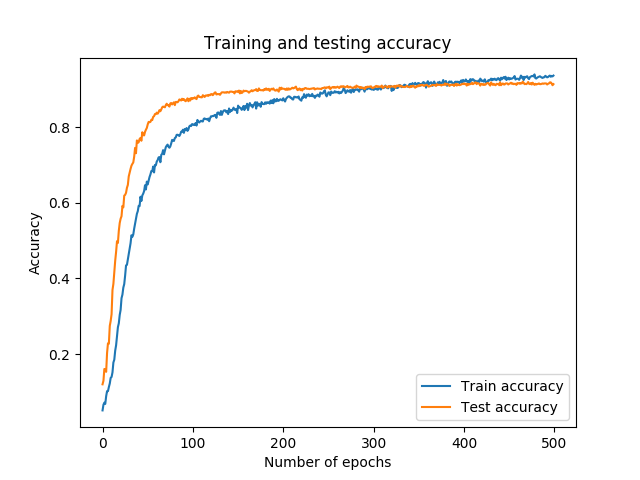
\includegraphics[width=3in]{images/test_4}
\caption{Training and cross-validation accuracy with a dropout of 50\%.}
\label{results_4}
\end{figure}

Smaller and bigger networks were also tested (as it can be seen in tables \ref{table:network_configuration_smaller} and \ref{table:network_configuration_bigger}), but the results were worse than with the previous network configurations (as it can be seen in the figures \ref{results_5} and \ref{results_6}, with the maximum accuracy of 12.70\% and 90.87\%).

\begin{figure}[!t]
\centering
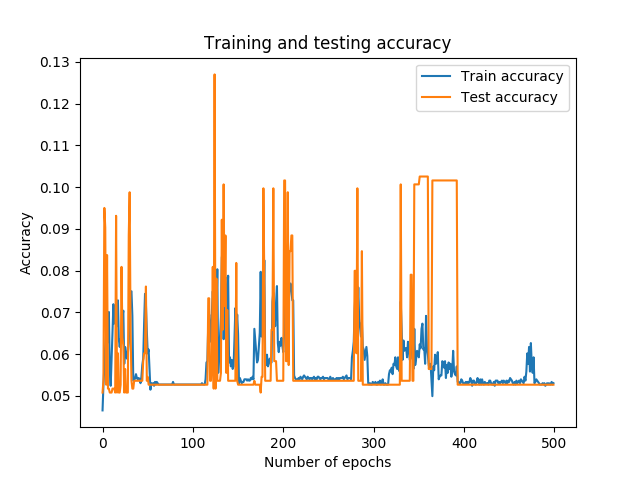
\includegraphics[width=3in]{images/test_5}
\caption{Training and cross-validation accuracy for a smaller network configuration.}
\label{results_5}
\end{figure}

\begin{figure}[!t]
\centering
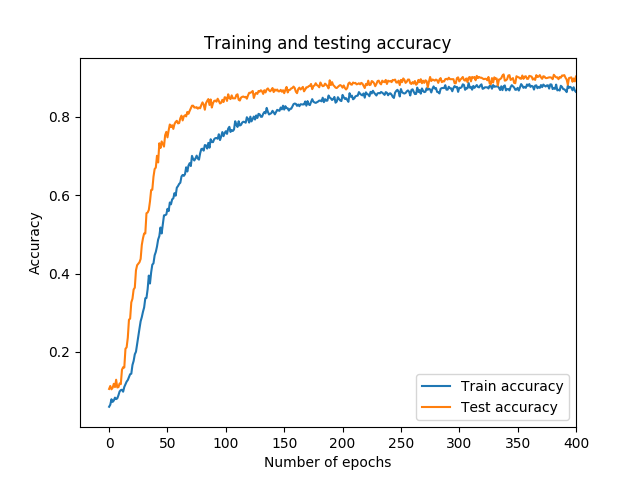
\includegraphics[width=3in]{images/test_6}
\caption{Training and cross-validation accuracy for a larger network configuration.}
\label{results_6}
\end{figure}

\begin{table}[]
\centering
\caption{Smaller network configuration.}
\label{table:network_configuration_smaller}
\begin{tabular}{|l|l|l|}
\hline
\textbf{Layer Type}   & \textbf{Neurons} & \textbf{Kernel Size} \\ \hline
Convolutional Layer   & 256              & 3x3                  \\ \hline
Pooling Layer         &                  & 2x2                  \\ \hline
Dropout (0.50)        &                  &                      \\ \hline
Convolutional Layer   & 512              & 3x3                  \\ \hline
Pooling Layer         &                  & 2x2                  \\ \hline
Dropout (0.50)        &                  &                      \\ \hline
Fully-connected Layer & 512              &                      \\ \hline
Dropout (0.50)        &                  &                      \\ \hline
Fully-connected Layer & 512              &                      \\ \hline
Output Layer          & 19               &                      \\ \hline
\end{tabular}
\end{table}

\begin{table}[]
\centering
\caption{Bigger network configuration.}
\label{table:network_configuration_bigger}
\begin{tabular}{|l|l|l|}
\hline
\textbf{Layer Type}   & \textbf{Neurons} & \textbf{Kernel Size} \\ \hline
Convolutional Layer   & 256              & 3x3                  \\ \hline
Convolutional Layer   & 256              & 3x3                  \\ \hline
Convolutional Layer   & 256              & 3x3                  \\ \hline
Pooling Layer         &                  & 2x2                  \\ \hline
Dropout (0.50)        &                  &                      \\ \hline
Convolutional Layer   & 512              & 3x3                  \\ \hline
Convolutional Layer   & 512              & 3x3                  \\ \hline
Convolutional Layer   & 512              & 3x3                  \\ \hline
Pooling Layer         &                  & 2x2                  \\ \hline
Dropout (0.50)        &                  &                      \\ \hline
Fully-connected Layer & 512              &                      \\ \hline
Fully-connected Layer & 512              &                      \\ \hline
Dropout (0.50)        &                  &                      \\ \hline
Fully-connected Layer & 512              &                      \\ \hline
Fully-connected Layer & 512              &                      \\ \hline
Output Layer          & 19               &                      \\ \hline
\end{tabular}
\end{table}

\subsection{Training using EMNIST dataset}

A possible way to increase the general accuracy of the model is to increase the number of training examples. That can be done using another dataset with more training examples and use the cross-validation set of the original CAPTCHA dataset to get the cross-validation accuracy. It is needed a dataset with all the 19 characters in the CAPTCHAs dataset. The EMNIST \cite{DBLP:journals/corr/CohenATS17} is an extension to the original MNIST dataset, with digits and letters. Only the 19 characters in the CAPTCHAs dataset are used from the EMNIST dataset. The frequency of each character in the EMNIST dataset is 2400. All characters have the same frequency.

The network configuration is described in table \ref{table:network_configuration_best} with 50\% of dropout and results are shown in the image \ref{results_7}. The highest accuracy achieved was 39.51\% for the cross-validation set. There are some possible explanations for why the cross-validation accuracy is much lower than the training accuracy (the model is underfitted). Due to the different dataset used, it can be possible that the difference between the characters in the EMNIST and in the CAPTCHAs dataset is too big for the model to be able to differentiate clearly the different characters. Besides that, the characters in the CAPTCHAs dataset all use the same font, which eases the recognition when trained with the same dataset, while the EMNIST dataset uses handwritten characters. It can be concluded that if it is desired to improve the accuracy in the CAPTCHAs dataset by increasing the training set, the best way to do that is to use the same dataset in the training and cross-validation set, but make modifications in the training set to increase the number of examples.

\begin{figure}[!t]
\centering
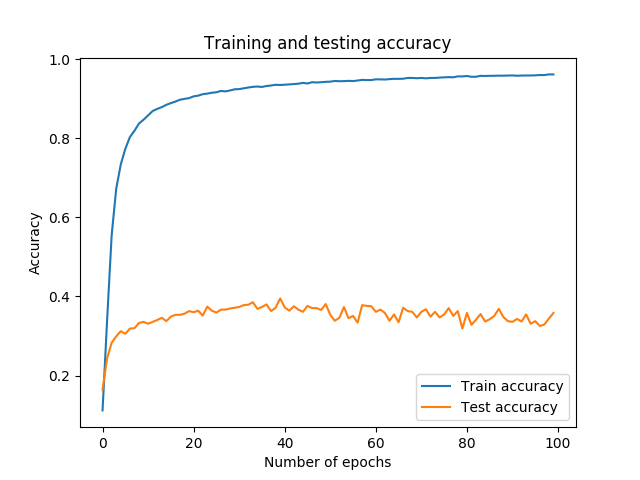
\includegraphics[width=3in]{images/test_7}
\caption{Training and cross-validation accuracy for training with the EMNIST dataset and testing with the CAPTCHAs dataset.}
\label{results_7}
\end{figure}

\subsection{Training with generated characters}

Due to the conclusions from the last subsection, the next step to improve the cross-validation accuracy is to generate more training examples based on the ones already existent. For this, two operations were applied to the images in the original training set: rotation and shifting.

To each example in the training set it was applied all combinations of rotations (-10º, 0º, 10º) and vertical (-3px, 0px, 3px) and horizontal (-3px, 0px, 3px) shifts. For each original example, they generated 27 images with the combinations of the image operations. A sample of the 27 images created for a character can be seen in figure \ref{generated_images}. The training set grew to 87048 examples among all characters (initially the training set had 3224 examples).

\begin{figure}[!t]
\centering
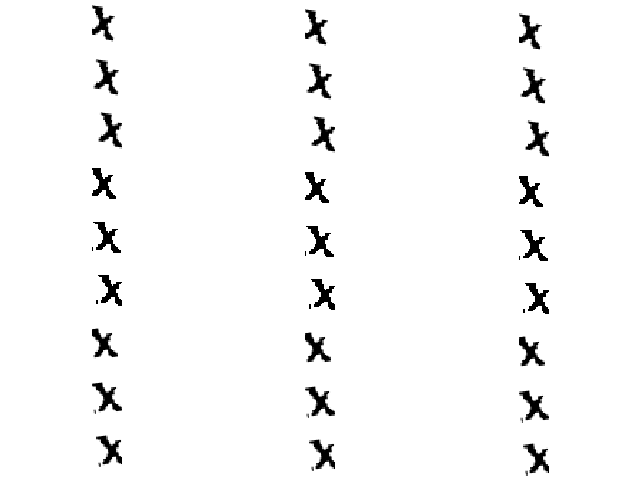
\includegraphics[width=3in]{images/generated_images}
\caption{27 generated images based on an image for the character 'x'.}
\label{generated_images}
\end{figure}

As it can be seen in the figure \ref{results_8}, the cross-validation accuracy is close to the training accuracy, reaching a maximum accuracy of 93.60\%.

\begin{figure}[!t]
\centering
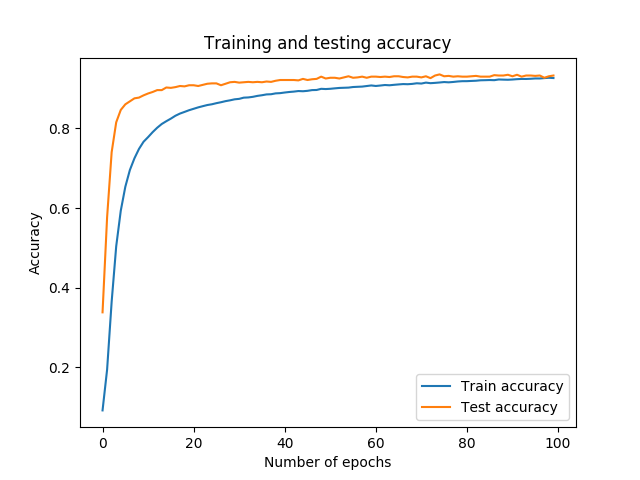
\includegraphics[width=3in]{images/test_8}
\caption{Training and cross-validation accuracy with generated images derived from the original training images for training.}
\label{results_8}
\end{figure}


\section{Final Results}

To get the final results, the model with the best cross-validation accuracy was chosen. In this case, the approach chosen was to generate images, based on the training and cross-validation set, for training, as described in the last section, and test with the test set. The results can be seen in figure \ref{results_9}, with a maximum accuracy of 93.91\%.

To obtain the accuracy of recognizing an entire CAPTCHA, a rough approximation can be made, following some assumptions. If it is assumed that the probability of a recognizing a character is independent of its position in the CAPTCHA and independent of the other characters in the CAPTCHA, the probability of correctly recognizing the text in a CAPTCHA can be calculated by

\[ p(CAPTCHA) = p(c_{1})*p(c_{2})*p(c_{3})*p(c_{4})*p(c_{5}) \]

being $p(c_{x})$ the probability of recognizing the character in the position x.

If it is assumed that all characters have the same probability of being recognized, the probability of correctly recognizing the text in a CAPTCHA can be calculated by

\[ p(CAPTCHA) = p(c)^5 \]

being $p(c)$ the probability of recognizing any character.

In this case, $p(c)$ is the obtained accuracy. So, the probability of correctly recognizing the text in a CAPTCHA is 73.04\%.

\begin{figure}[!t]
\centering
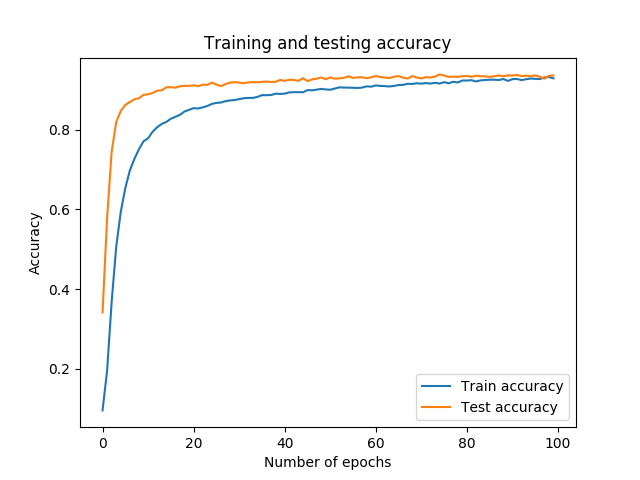
\includegraphics[width=3in]{images/test_9}
\caption{Final training and test accuracy for the model with the best cross-validation results.}
\label{results_9}
\end{figure}


\section{Visualizing the learning in the convolutional layers}

Since 2013, a wide array of techniques have been developed for visualizing and interpreting the internals of a Convolutional Neural Network \cite{10.1007/978-3-319-10590-1_53}. These techniques are useful to understand what is the network learning, to improve the network in future iterations.

Firstly, it will be shown the intermediate activations of the network, displaying the outputs of the four convolutional layers in the network given a certain input. The activation image is an image with the character '4'. The four convolutional layers described in the architecture of the network (table \ref{table:network_configuration_best}) are depicted in the figures \ref{activation_1}, \ref{activation_2}, \ref{activation_3} and \ref{activation_4}.

\begin{figure}[!t]
\centering
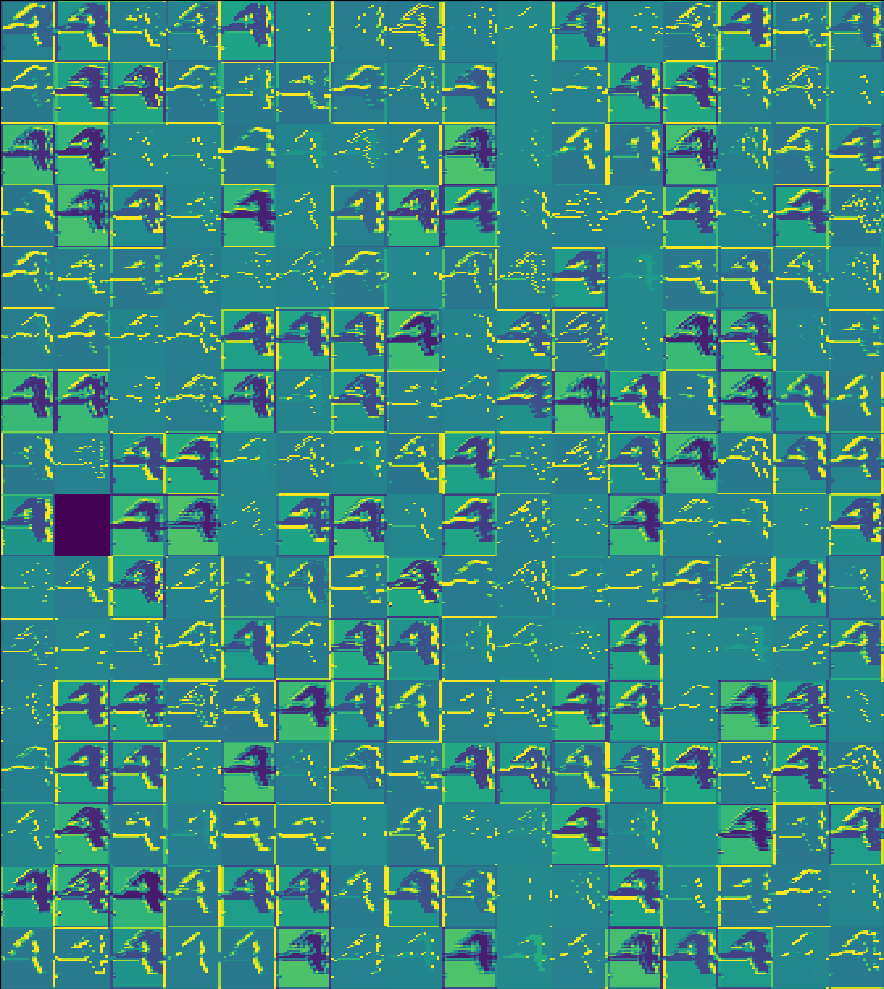
\includegraphics[width=3in]{images/activation_conv1_4.png}
\caption{Activations of the first convolutional layer of the network, given an image with the character '4'.}
\label{activation_1}
\end{figure}

\begin{figure}[!t]
\centering
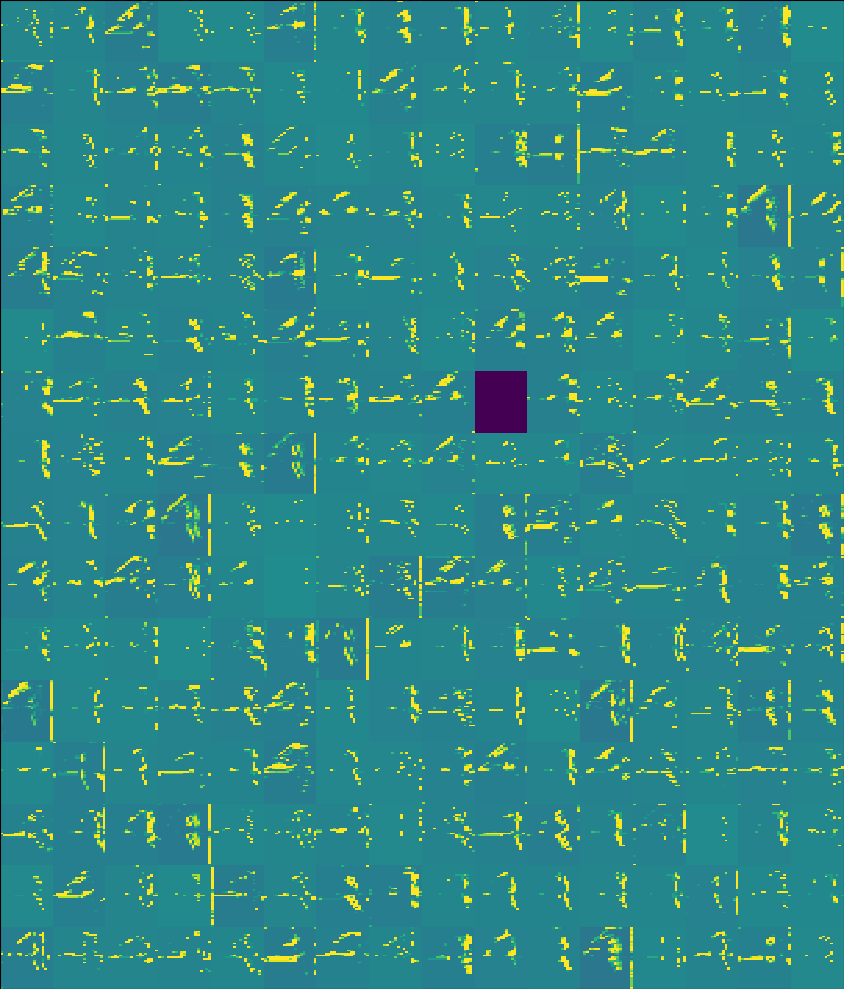
\includegraphics[width=3in]{images/activation_conv2_4.png}
\caption{Activations of the second convolutional layer of the network, given an image with the character '4'.}
\label{activation_2}
\end{figure}

\begin{figure}[!t]
\centering
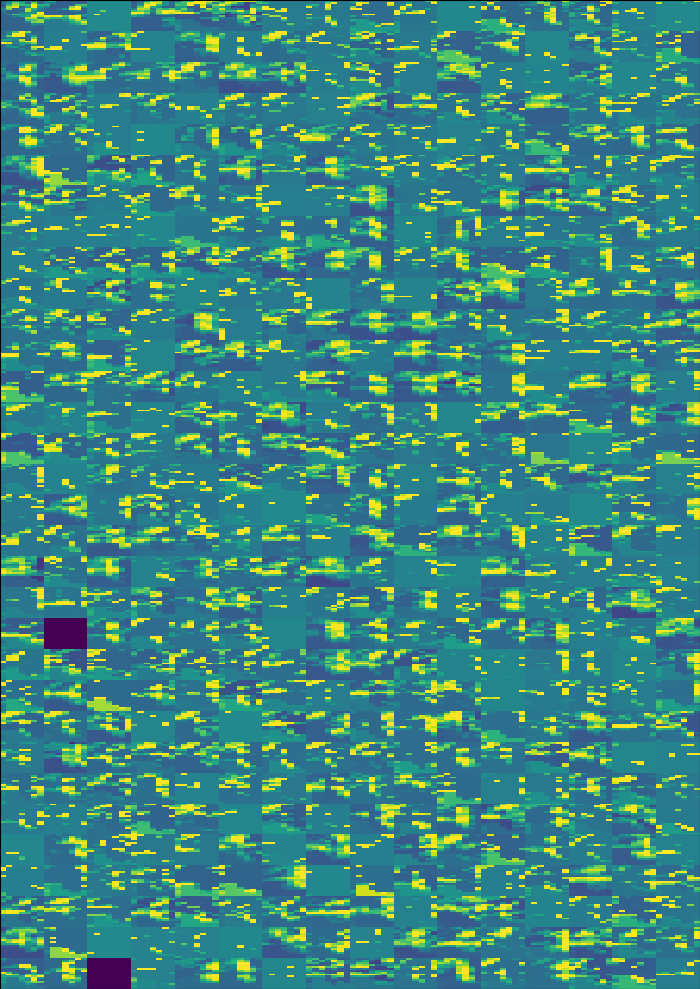
\includegraphics[width=3in]{images/activation_conv3_4.png}
\caption{Activations of the third convolutional layer of the network, given an image with the character '4'.}
\label{activation_3}
\end{figure}

\begin{figure}[!t]
\centering
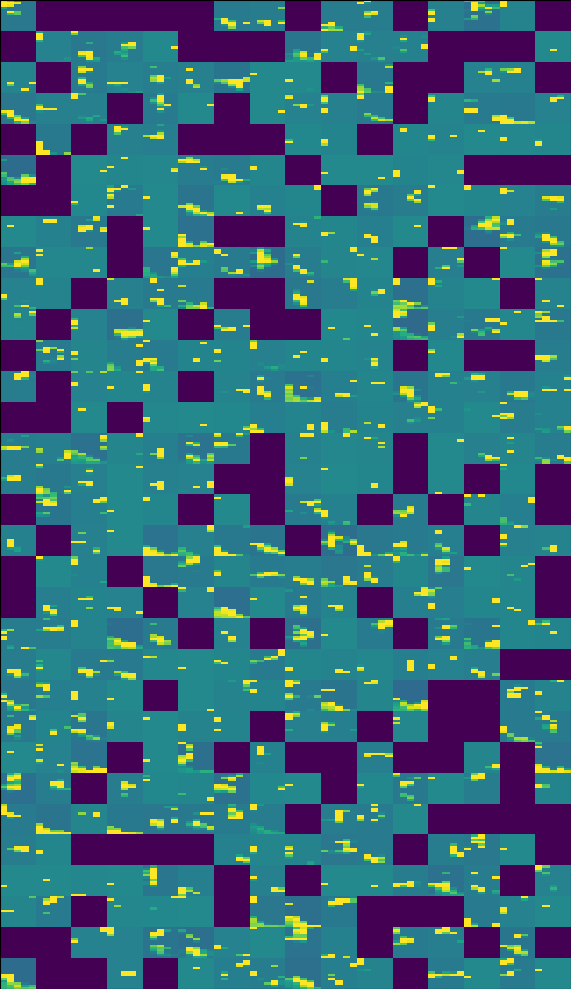
\includegraphics[width=3in]{images/activation_conv4_4.png}
\caption{Activations of the last convolutional layer of the network, given an image with the character '4'.}
\label{activation_4}
\end{figure}

As expected, the first layer contains a collection of edge detectors, and the activations retain a big part of the information in the figure. As it goes deeper into the network, the activations become less interpretable and more abstract. Higher-level concepts are being created by the network. It also can be seen that more filters are "blank", which means that they are not activated by the input image. This happens because deeper layers are more specialized in specific patterns than the initial ones.

It is also useful to visualize the convolutional filters, to understand exactly what pattern each filter is detecting. To do that, it can be used the technique of \textit{gradient ascent in input space}\cite{Yosinski2015UnderstandingNN}: applying gradient descent to the input image so as to maximize the response of a filter, starting from a random image. The first 64 filter patterns of each of the four convolutional layers in the network can be seen in the figures \ref{first_layer_patterns}, \ref{second_layer_patterns}, \ref{third_layer_patterns} and \ref{fourth_layer_patterns}.

\begin{figure}[!t]
\centering
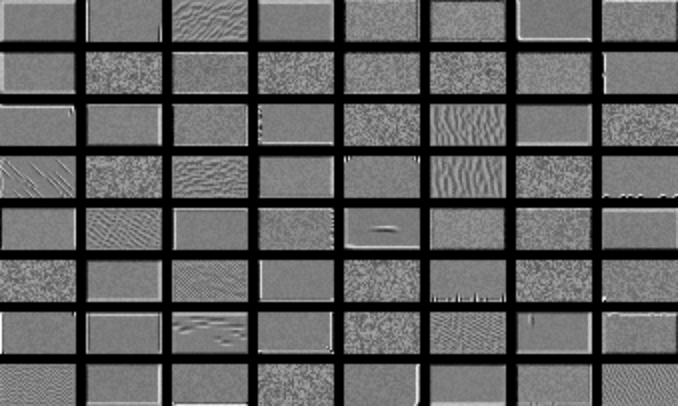
\includegraphics[width=3in]{images/conv2d_1_filter_activation.png}
\caption{Filter patterns for the first convolutional layer of the network.}
\label{first_layer_patterns}
\end{figure}

\begin{figure}[!t]
\centering
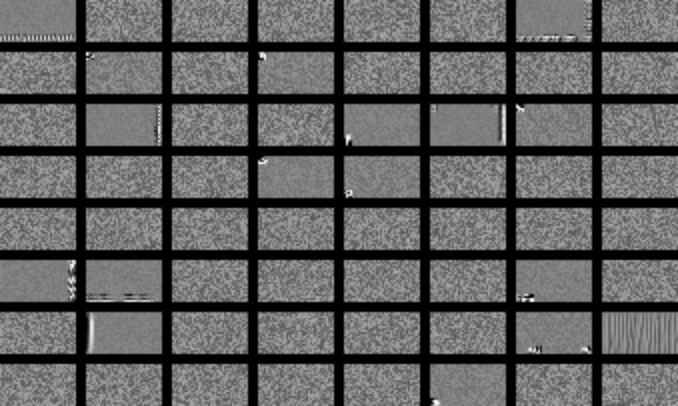
\includegraphics[width=3in]{images/conv2d_2_filter_activation.png}
\caption{Filter patterns for the second convolutional layer of the network.}
\label{second_layer_patterns}
\end{figure}


\begin{figure}[!t]
\centering
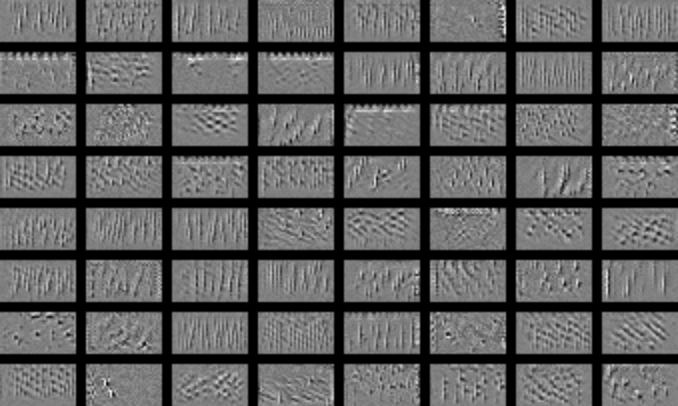
\includegraphics[width=3in]{images/conv2d_3_filter_activation.png}
\caption{Filter patterns for the third convolutional layer of the network.}
\label{third_layer_patterns}
\end{figure}

\begin{figure}[!t]
\centering
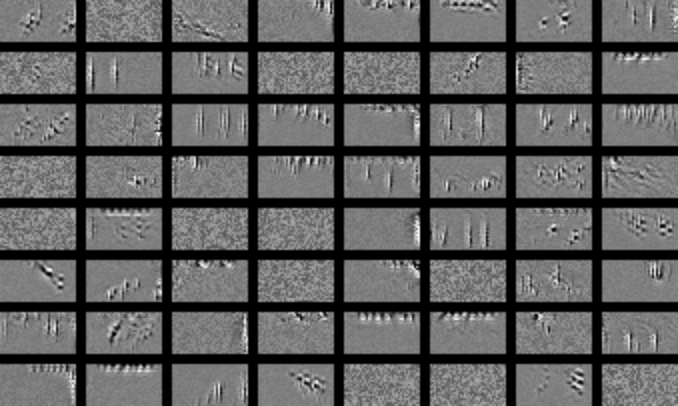
\includegraphics[width=3in]{images/conv2d_4_filter_activation.png}
\caption{Filter patterns for the last convolutional layer of the network.}
\label{fourth_layer_patterns}
\end{figure}

As can be seen, the filters of the first layer detect vertical, horizontal and diagonal patterns, which was expected due to the activations of the first convolutional layer (figure \ref{activation_1}). Deeper layers encode more abstract textures, some of them with resemblance to parts of characters in the dataset.

Finally, it was applied a technique called Class Activation Map (CAM) visualization, that produces heat maps of class activation over images. The implementation was explained in \cite{Selvaraju2017} and the output image represents how important each location is with respect to the class under consideration. According to the output of the network, it will be created a heat map that highlights the most important location that leads to the network deciding on that output. The figure \ref{heatmap} shows the heat map for a member of each class in the dataset.

\begin{figure}[!t]
\centering
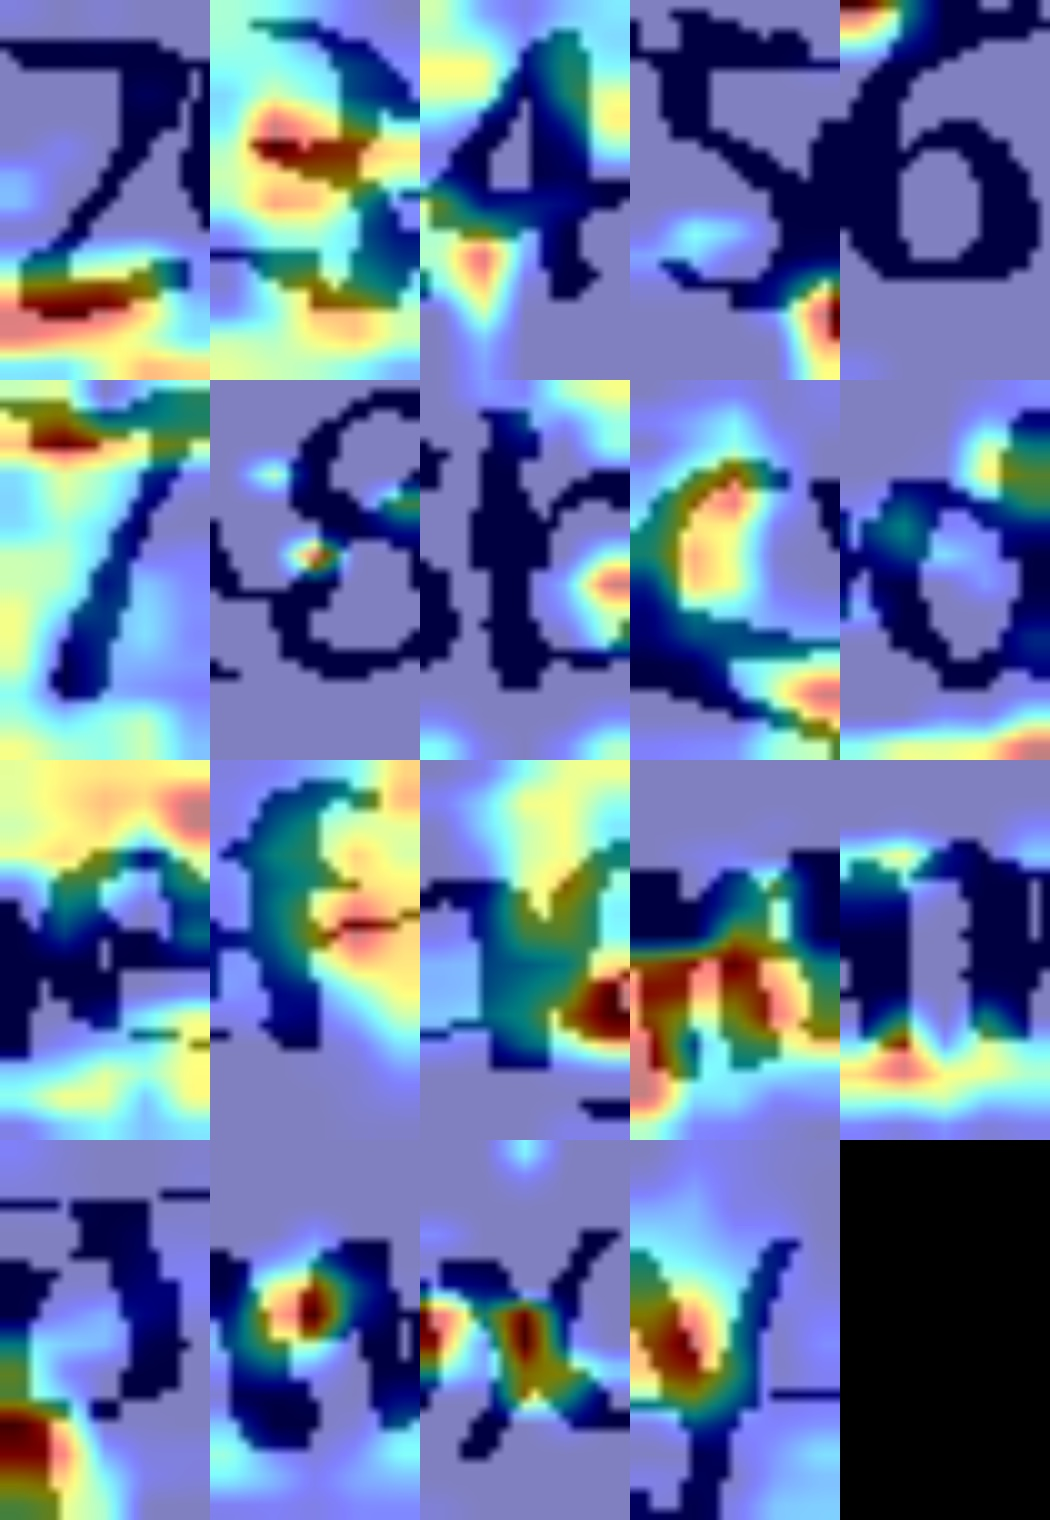
\includegraphics[width=3in]{images/heatmaps}
\caption{Heat map detailing the most important locations of an image for the classification given by the network.}
\label{heatmap}
\end{figure}

It is interesting how, for some characters, the network seems to give more importance to the white space around the character than the character itself, as it can be seen in the heat map for the characters '4', 'e', '5' or '6'. However, for most characters, the heat map is understandable and the network focuses on the particular strokes of each character, as it can be seen for characters '2', '3', 'm', 'x' or 'y'. 

\section{Conclusion \& Future Work}

On this report, it was shown that the CAPTCHA recognition problem can be easily solved when the character segmentation is done effectively with no errors. It achieved a final accuracy of 93.91\% of character recognition on the used dataset.

Another possible technique to improve the current accuracy of the model to character recognition is to explore the recent advances in transfer learning with a bigger dataset. Although another dataset was used for training in one of the approaches, other approaches can be made to achieve better accuracy with transfer learning, such as training just the initial layers with the bigger dataset and retraining only the last layers with the dataset from the problem. Such approach was not taken due to the specificity of the task. Because most pre-trained datasets are suitable for object recognition, with RGB colour, for bigger images, it was opted not to go for that approach, believing that data augmentation (image generation) would prove itself to achieve higher accuracy (as it did). However, it is an approach that is worth exploring in the future.

It was also shown that the generation of new images to include in the training set with slight modifications, such as rotations or translations, improves the accuracy of the model, especially when the training set is small.



% if have a single appendix:
%\appendix[Proof of the Zonklar Equations]
% or
%\appendix  % for no appendix heading
% do not use \section anymore after \appendix, only \section*
% is possibly needed

% use appendices with more than one appendix
% then use \section to start each appendix
% you must declare a \section before using any
% \subsection or using \label (\appendices by itself
% starts a section numbered zero.)
%



%\section{Proof of the First Zonklar Equation}
%Appendix one text goes here.

% you can choose not to have a title for an appendix
% if you want by leaving the argument blank
%\section{}
%Appendix two text goes here.


% use section* for acknowledgment
%\section*{Acknowledgment}


%The authors would like to thank...


% Can use something like this to put references on a page
% by themselves when using endfloat and the captionsoff option.
\ifCLASSOPTIONcaptionsoff
  \newpage
\fi



% trigger a \newpage just before the given reference
% number - used to balance the columns on the last page
% adjust value as needed - may need to be readjusted if
% the document is modified later
%\IEEEtriggeratref{8}
% The "triggered" command can be changed if desired:
%\IEEEtriggercmd{\enlargethispage{-5in}}

% references section

% can use a bibliography generated by BibTeX as a .bbl file
% BibTeX documentation can be easily obtained at:
% http://mirror.ctan.org/biblio/bibtex/contrib/doc/
% The IEEEtran BibTeX style support page is at:
% http://www.michaelshell.org/tex/ieeetran/bibtex
%\bibliographystyle{plainnat}
\bibliographystyle{IEEEtran}
% argument is your BibTeX string definitions and bibliography database(s)
\bibliography{captcha_references.bib}
%
% <OR> manually copy in the resultant .bbl file
% set second argument of \begin to the number of references
% (used to reserve space for the reference number labels box)
%\begin{thebibliography}

% \bibitem{IEEEhowto:kopka}
% H.~Kopka and P.~W. Daly, \emph{A Guide to \LaTeX}, 3rd~ed.\hskip 1em plus
%   0.5em minus 0.4em\relax Harlow, England: Addison-Wesley, 1999.

%\end{thebibliography}

% biography section
% 
% If you have an EPS/PDF photo (graphicx package needed) extra braces are
% needed around the contents of the optional argument to biography to prevent
% the LaTeX parser from getting confused when it sees the complicated
% \includegraphics command within an optional argument. (You could create
% your own custom macro containing the \includegraphics command to make things
% simpler here.)
%\begin{IEEEbiography}[{\includegraphics[width=1in,height=1.25in,clip,keepaspectratio]{mshell}}]{Michael Shell}
% or if you just want to reserve a space for a photo:

% \begin{IEEEbiography}{Michael Shell}
% Biography text here.
% \end{IEEEbiography}

% if you will not have a photo at all:
% \begin{IEEEbiographynophoto}{John Doe}
% Biography text here.
% \end{IEEEbiographynophoto}

% insert where needed to balance the two columns on the last page with
% biographies
%\newpage

%\begin{IEEEbiographynophoto}{Jane Doe}

%\end{IEEEbiographynophoto}

% You can push biographies down or up by placing
% a \vfill before or after them. The appropriate
% use of \vfill depends on what kind of text is
% on the last page and whether or not the columns
% are being equalized.

%\vfill

% Can be used to pull up biographies so that the bottom of the last one
% is flush with the other column.
%\enlargethispage{-5in}



% that's all folks
\end{document}
